\section{Ziel}
\label{sec:Ziel}

Versuchsziel ist es, Brennweiten verschiedener Linsen sowohl mit Hilfe der Linsengleichung als auch mit der Methode nach \textsc{Bessel} zu berechnen. 
Außerdem werden Brennweite und Lage der Hauptebenen eines Linsensystems mit der Methode nach \textsc{Abbe} bestimmt.
\section{Theorie}
\label{sec:theorie}
Nach der geometrischen Optik breitet sich Licht in Form von Strahlen aus. 
Dies ist eine gültige Näherung, wenn alle Abmessungen einer Apparatur groß gegenüber der Wellenlänge des Lichtes sind. 
Tritt ein Lichtstrahl in ein Medium mit anderer optischer Dichte, wird er nach dem \textsc{Snellius}'schen Brechungsgesetz gebrochen. 
Diese Brechung wird für die Konstruktion von Linsen, deren Material die Dichte von Luft übersteigt, benützt.
In Abhängigkeit von der Dicke und Krümmung weisen Linsen verschiedene Eigenschaften auf. 

\emph{Sammellinsen} sind konvex gekrümmt und bündeln parallel eintreffende Lichtstrahlen im Brennpunkt. Dieser Brennpunkt befindet sich im Abstand $f$, der Brennweite, von der Mittelebene entfernt. 
Wird ein Gegenstand im Abstand der doppelten Brennweite von der Linse aufgestellt, entsteht im gleichen Abstand auf der anderen Seite der Linse ein reelles Bild von dem Objekt. 
Im Allgemeinen wird der Abstand zwischen Linsenmittelachse und Bild als \emph{Bildweite} $b$, der Abstand zwischen Linsenmittelachse und Gegenstand als \emph{Gegenstandsweite} $g$ bezeichnet. 
Beide Größen $b$, $g$ sind Projektionsweiten und sind bei Sammellinsen positiv.\\
\emph{Zerstreuungslinsen} sind konkav gekrümmt und zerstreuen parallel auftreffende Lichtstrahlen. 
Der virtuelle Schnittpunkt der Lichtstahlen, die als parallele Lichtstrahlen von der Linse zerstreut wurden, ist der virtuelle Brennpunkt der Linse.
Bei Zerstreuungslinsen sind Projektions- und Brennweite negativ.\\
Anders als bei dünnen Linsen geschieht die Brechung bei einer dicken Linse an zwei Hauptebenen, $H$ und $H'$, da der Strahl einen weiteren Weg im Medium zurücklegt.
Relativ zu den Hauptebenen sind, wie in Abbildung \ref{fig:strahlengaenge} erkennbar, $b$, $b'$ und $g$, $g'$ die kennzeichnenden Größen der Linse. 
Der Strahlengang wird durch Parallel-, Brennpunkt- und Mittelpunktstrahl wie in Abbildung \ref{fig:strahlengaenge} dargestellt.

Durchquert ein Lichtstrahl eine dünne Linse, wird er an der Mittelebene gebrochen.
Die Brechkraft $D$ -- der Kehrwert der Brennweite $f$ mit der Einheit $ \mathrm{dpt}=\sfrac{1}{\si{\meter}}$ -- kann für dünne Linsen berechnet werden mit der \emph{Linsengleichung}
\begin{equation}
	D=\frac{1}{f}=\frac{1}{b}+\frac{1}{g}.
	\label{eq:linsengleichung}
\end{equation}
\newpage
Über das \emph{Abbildungsgesetz} 
\begin{equation}
	V=\frac{B}{G}=\frac{b}{g}
\end{equation}
mit Bildgröße $B$ und Gegenstandsgröße $G$ wird die Bildvergrößerung $V$ bestimmt.

Es treten bei der Verwendung von Linsen \emph{Abbildungsfehler} auf. 
Die Nährung der geometrischen Optik gilt nur für achsennahe Strahlen, achsenferne Strahlen befinden sich weit von der optischen Achse eines Systems entfernt und werden stärker gebrochen. 
Dadurch liegt der Brennpunkt der achsenfernen Strahlen nicht auf dem Brennpunkt der achsennahen Strahlen, wodurch nicht das gesamte Licht durch die Linse scharf abgebildet wird. Dieses Phänomen wird \emph{sphärische Aberration} genannt.\\
Ist die optische Dichte des Linsenmaterials abhängig von der Wellenlänge des Lichtes, kommt es zur \emph{chromatischen Aberration}. 
Wird nicht-monochromatisches Licht durch eine Linse geschickt, liegen die Brennpunkte der einzelnen Lichtfarben nicht übereinander, wodurch ein unscharfes Bild entsteht.

\subsection{Brennweitenbestimmung nach \texorpdfstring{\textsc{Bessel}}{Bessel}}
\label{sec:theorie1}
Ist der Abstand $e=g+b$ zwischen Gegenstand und Schirm konstant und größer als die vierfache Brennweite $f$ der Linse, lassen sich zwei Linsenpositionen finden, die ein scharfes Bild erzeugen. 
Dabei sind die zwei paarweise gefundenen Gegenstands- und Bildweiten symmetrisch, es gilt
\begin{equation}
	b_1=g_2 \qquad \text{und} \qquad b_2=g_1.
\end{equation}

Mit der Differenz der Projektionsweiten $d= g-b$ gilt weiter
\begin{equation}
	f=\frac{e²-d²}{4e}.
\end{equation}

\subsection{Bestimmung der Lage von Hauptachsen nach \texorpdfstring{\textsc{Abbe}}{Abbe}}
\label{sec:theorie2}
\begin{figure}[h!]
	\begin{minipage}[r,t]{0.6\textwidth}
		Über die Methode von \textsc{Abbe} können dicke Linsen oder Linsensysteme auf die Lage der Hauptachsen $H$, $H'$ und Gesamtbrennweite $f$ untersucht werden. 
		Es gelten die Beziehungen
		\begin{subequations}
			\begin{align}
			g'&=g+h =f\cdot\biggl(1+\frac{1}{V}\biggr)+h
			\end{align}
			\begin{align}
			b'&=b+h' =f\cdot(1+V)+h',
			\end{align}
			\label{eq:abbe}
		\end{subequations}
	\end{minipage}
	\begin{minipage}[l,t]{0.4\textwidth}
		\hfill
		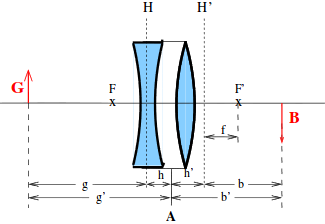
\includegraphics[width=\textwidth]{Bilder/dickelinseHELENA.png}
		\caption{Bezeichnung an einem Linsensystem. \cite{skript}}
		\label{fig:label}
	\end{minipage}
\end{figure}
welche bei bekannter Vergrößerung $V$ sowie Bild- und Gegenstandsweiten $g'$ und $b'$ bezogen auf einen festen Punkt des Linsensystems, Aussagen über die Lage der Hauptachsen zulassen. 
\vspace{1cm}
\begin{figure}[hb]
	\centering
	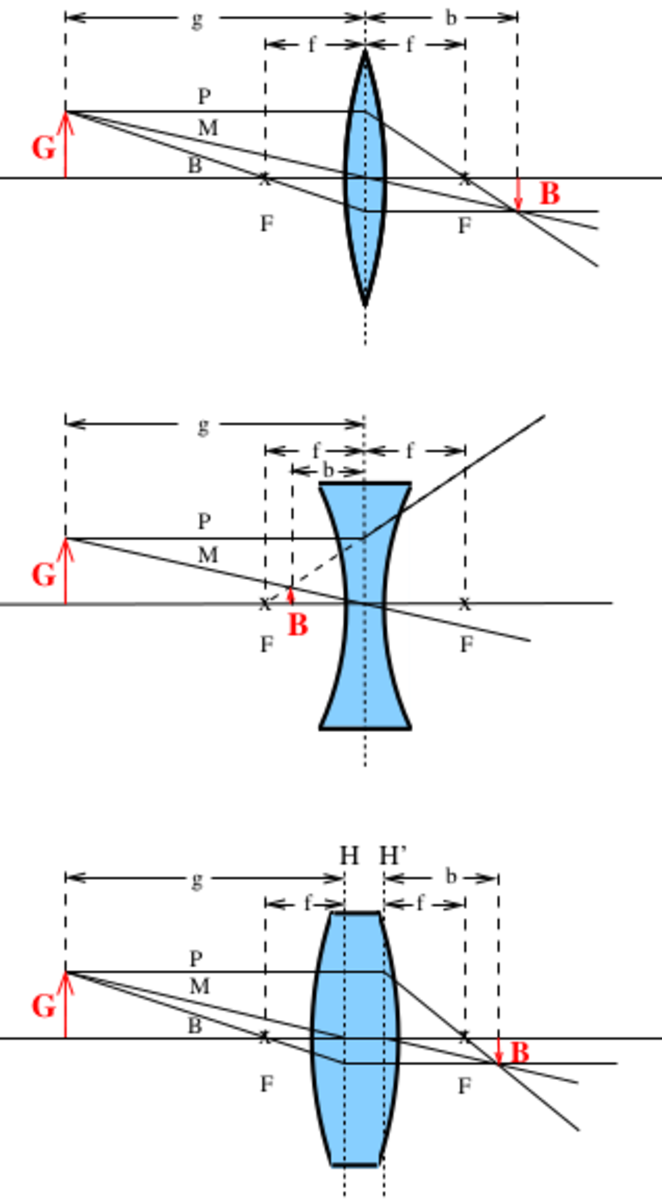
\includegraphics[width=0.55\textwidth]{Bilder/Bildkonstruktionen.pdf}
	\caption{Strahlengänge verschiedener Linsen (von oben nach unten: Sammellinse, Zerstreuungslinse, dicke (Sammel-)linse). \cite{skript}}
	\label{fig:strahlengaenge}
\end{figure}